\documentclass[a4paper]{article}
%\usepackage{exercise}
%um nur aufgaben zu zeigen
\usepackage[noanswer]{exercise} 
\usepackage{../images/preamble}
\usepackage{rotating}
\usetikzlibrary{decorations.pathmorphing}
\usetikzlibrary{decorations.markings}
\usetikzlibrary{arrows}
\usetikzlibrary{shapes.geometric}
\newcommand{\midarrow}{\tikz \draw[-triangle 90] (0,0) -- +(.02,0);}
\usepackage{xcolor}
%\usepackage{draftwatermark}
%\SetWatermarkText{\textsc{Draft 2}}
%\SetWatermarkScale{3}
%\SetWatermarkColor{red!30}


\usepackage[printwatermark]{xwatermark}
%\newsavebox\mybox
%\savebox\mybox{\tikz[color=red,opacity=0.3]\node{\textsc{Entwurf}};}
%\newwatermark*[
%allpages,
%angle=45,
%scale=10,
%xpos=-4cm,
%ypos=4cm
%]{\usebox\mybox}
\pagestyle{fancy}
\fancyhead[L]{
\includegraphics[width=2cm]{../images/logo_scaled.pdf}}
\fancyhead[R]{\textsc{Aufgabenserie 8}}


\begin{document}
	\vspace*{-1cm}
	\parbox{4cm}{\vspace{-0.2cm}
\includegraphics[width=5cm]{../images/logo_scaled.pdf}}
	\parbox{10.6cm}{\setstretch{2.0} \centering{ \huge \textsf{Aufgabenserie 8
			}}\\
			%Abgabe: 8. April 2018 \\ 
			\vspace*{0.3cm} }
		\vspace{0.5cm}

\thispagestyle{empty}
\begin{framed}
	\noindent
	\scriptsize
	 Lösungen könnt ihr an \href{mailto:physikrolf@gmail.com}{physikrolf@gmail.com} schicken.
	 Neue Aufgaben wird es dann vermutlich wieder Ende Juni geben.
	 \\ Die aktuellen Aufgaben sowie alle alten Aufgabenserien findet ihr auch auf \url{pankratius.github.io/rolf}.
\end{framed}

\noindent

\begin{Exercise}[title = Ionen im Magnetfeld, origin = 8. IPhO 1975, difficulty = 4, label = ions]
	\begin{center}	
		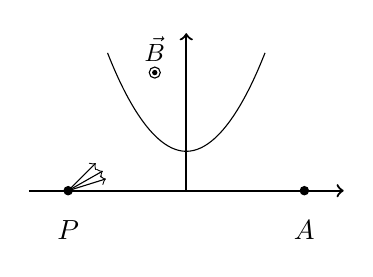
\begin{tikzpicture}
		\draw[thick,->] (-2,0) -- (2,0);
		\draw[thick,->] (0,0) -- (0,2);
		\filldraw[black] (-1.5,0) circle (1.5pt);
		\filldraw[black] (1.5,0) circle (1.5pt);
		\node at (-1.5,-.5) {$P$};
		\node at (1.5,-.5) {$A$};
		\draw[->] (-1.5,0) -- (-1.15,.35);
		\draw[->] (-1.5,0) -- (-1.06,0.25);
		\draw[->] (-1.5,0) -- (-1.02,0.15);
		\draw (0,.5) parabola (1,1.75);
		\draw (0,.5) parabola (-1,1.75);
		\filldraw[black] (-.4,1.5) circle (.75pt);
		\draw (-.4,1.5) circle (2pt);
		\node at (-.4,1.8) {\small $\vec{B}$};
		\end{tikzpicture}\\
	\end{center}
	Ein Strahl positiv geladener Ionen der Ladung $+e$ und der Masse $m$ breitet sich vom Punkt $P$ gleichmäßig in alle Richtungen aus. Dabei wurden die Ionen zuvor mit einer Spannung $U$ beschleunigt.\\
	In der Ebene der Elektroenenausbreitung befindet sich nun ein homogenes Magnetfeld der Stärke $B$, welches senkrecht auf dieser steht. Die Begrenzungslinien des Magnetfeldes sind gerade so, dass die anfangs im Punkt $P$ diviergierenden Ionen im Punkt $A$ wieder fokusiert werden. Wir wollen diese Begrenzungslinien nun näher beschreiben.\\
	Dazu nehmen wir an, dass die Ionenbahn spiegelsymmetrisch zur Mittelsenkrechten auf $\overline{PA}$ ist. Gleichzeitig sollen sowohl $P$ und $A$ nicht im Magnetfeld liegen. 
	\begin{enumerate}[a)]
		\item Berechne den Krümmungsradius einer Ionenbahn in Abhängigkeit von $U$ und $B$, sowie auftretender Konstanten.
		\item Beschreibe charakterstische Eigenschaften der Ionenbahn in diesem System.
		\item Konstruiere die Begrenzungslinien des Magnetfeldes für die Fälle $R<a$, $R=a$ und $R>a$. 	Dabei ist $a = \overline{PA}/2$.
		\item Finde eine Gleichung, die diese Begrenzungslinien beschreibt.
	\end{enumerate}

\end{Exercise}
\begin{minipage}[b]{0.65\textwidth}
\begin{Exercise}[title = rutschender Zylinder, origin = EstPho 2016, difficulty = 3, label = cylinder]
 Ein Zylinder der Masse $m$ und mit dem Radius $R$ rutscht auf einer Platte mit einer Geschwindigkeit $v$ und einer Winkelgeschwindigkeit $\omega$. Nachdem der Zylinder aufhört zu rutschen, bewegt er sich mit einer Geschwindigkeit $v$ in die entgegengesetze Richtung. Wie groß war $\omega$?
\end{Exercise}
\end{minipage}
\begin{minipage}[t]{0.35\textwidth}
	\centering
	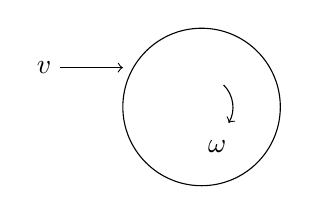
\begin{tikzpicture}
	\draw (0,0) circle (1);
	\draw[->] (-1.8,.5) -- (-1,.5);
	\node at (-2,.5) {$v$};
	\draw[->] (0.28,0.28) arc (45:-30:.4);
	\node at (.2,-.5) {$\omega$};
	\end{tikzpicture}
\end{minipage}

\begin{minipage}[b]{0.65\textwidth}
\begin{Exercise}[title = Polygon, origin = P. Gnädig, difficulty = 2, label = polygrav]
	Wir betrachten ein regelmäßiges n-Eck, bei dem an jeder Ecke eine Masse $m$ sitzt. Wie bewegt sich das System, wenn nur die Gravitationskraft zwischen den Körpern wirkt? Wie viel Zeit (in Abhänigkeit von $n$) vergeht, bis das System seinen Endzustand erreicht hat? 
\end{Exercise}
\end{minipage}
\begin{minipage}[b]{0.35\textwidth}
	\centering
	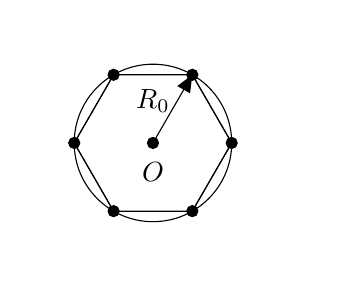
\begin{tikzpicture}[line cap=round,line join=round,>=triangle 45,x=1.0cm,y=1.0cm]
	\clip(-1.0911274272504616,-0.595261736026898) rectangle (2.4959243296533993,2.330040817448145);
	\draw(0.,0.) -- (1.,0.) -- (1.5,0.8660254037844387) -- (1.,1.7320508075688776) -- (0.,1.7320508075688779) -- (-0.5,0.8660254037844395) -- cycle;
	\draw (0.,0.)-- (1.,0.);
	\draw (1.,0.)-- (1.5,0.8660254037844387);
	\draw (1.5,0.8660254037844387)-- (1.,1.7320508075688776);
	\draw (1.,1.7320508075688776)-- (0.,1.7320508075688779);
	\draw (0.,1.7320508075688779)-- (-0.5,0.8660254037844395);
	\draw (-0.5,0.8660254037844395)-- (0.,0.);
	\draw(0.5,0.866025403784439) circle (1.cm);
	\draw [->] (0.5,0.866025403784439) -- (1.,1.7320508075688776);
	\begin{scriptsize}
	\draw [fill=black] (0.,0.) circle (2.0pt);
	\draw [fill=black] (1.,0.) circle (2.0pt);
	\draw [fill=black] (1.5,0.8660254037844387) circle (2.0pt);
	\draw [fill=black] (1.,1.7320508075688776) circle (2.0pt);
	\draw [fill=black] (0.,1.7320508075688779) circle (2.0pt);
	\draw [fill=black] (-0.5,0.8660254037844395) circle (2.0pt);
	\draw [fill=black] (0.5,0.866025403784439) circle (2.0pt);
	\end{scriptsize}
	\node at (0.5,1.4){$R_0$};
	\node at (0.5,0.5){$O$};
	\end{tikzpicture}
\end{minipage}
\begin{Answer}[ref = polygrav]
	Aus Symmetriegründen heben sich die nicht-radialen Teile der wirkenden Gravitationskräfte auf, sodass alle $n$ Massen sich zum Mittelpunkt des Polygons, $O$, bewegen. Dabei muss die polygonform erhalten bleiben. Weil die Abhängigkeit Körperabstand-Gravitationskraft aber nicht-linear ist, ist die Bewegung nicht gleichmäßig beschleunigt. Vielmehr sollte die Beschleunigung größer werden, je geringer der Körperabstand ist.\\
	Um nun die Zeit $T$ auszurechnen, bis die Körper im Punkt $O$ kollidieren, kann man zuerst die Kraft auf eine der Massen $m$ ausrechnen. Diese ist gegeben durch die Summe der Radialteile aller  Gravitationskräfte der anderen $n-1$ Körper, also, wenn der Radius des Polygons gerade $R$ ist,
	\begin{equation}\label{polygrav:f}
		F = Gm \sum_{i= 1}^{n-1}\frac{m \sin\left(\frac{\pi}{i}\right)}{\left(2R  \sin\left(\frac{\pi}{i}\right)\right)^2} = \frac{Gm}{R^2}\cdot \underbrace{ \frac{m}{4}\sum_{i=1}^{n-1} \frac{1}{\sin \frac{\pi}{i}}}_{:= M_n}.
 	\end{equation}
 	Die Kraft ist also so, als würde sich der Körper im Gravitationsfeld eines stationären Körpers mit der Masse $M_n = \frac{m}{4}\sum_{i=1}^{n-1} \frac{1}{\sin \frac{\pi}{i}}$ bewegen.\\
 	Diese Bewegung kann man jetzt als Bewegung entlang einer Ellipse ohne kleiner Halbachse, und mit großer Halbachse $\frac{R_0}{2}$ auffassen. Die Zeit, die dann bis zum Zusammensturz benötigt wird, entspricht genau der halben Periode $\nicefrac{T_e}{2}$. \\
 	Diese kann man über das dritte Keplersche Gesetz aus der entsprechenden Periode $T_k$ für eine Kreisbahn mit Radius $R_0$ ausrechen, wobei $F_g = F_{rad}$ benutzt wird:
 	\begin{equation}\label{polygrav:tc}
 		\frac{GmM_n}{R_0^2}  = m R\underbrace{\left(\frac{2\pi}{T_k}\right)^2}_{=\omega ^2} \Rightarrow T_k = 2\pi\sqrt{\frac{R_0^3}{GM_n}}.
 	\end{equation}
 	Mit dem dritten Keplerschen Gesetz folgt dann
 	\begin{equation}
 	\boxed{	\left(\frac{T_e}{T_k}\right)^2 = \left(\frac{\nicefrac{R_0}{2}}{R_0}\right)^3 \Rightarrow T_e = \pi \sqrt{\frac{R_0^3}{8GM_n}}.}
 	\end{equation}
\end{Answer}
 

\end{document}